%Préambule du document :
\documentclass[11pt]{article}
\usepackage[utf8]{inputenc}
\usepackage[french]{babel}
\usepackage{amsmath}
\usepackage{tikz}

%Corps du document :
\begin{document}
  \center 
\includegraphics[width=8cm]{logo.png}

\begin{center}
\textsc{\Large M1 Informatique - Projet ANDROIDE}\\[0.5cm]
\textsc{\Large  Carnet de bord }\\[0.5cm]
\textbf{Robotique adaptative en essaim: effet de l'environnement sur l'apprentissage de stratégies collectives} \\[3cm]
\end{center}


\begin{center}
Roza Amokrane\\[0.3cm]
Nabila Ould Belkacem\\[0.8cm]
\textbf{Encadrant:}\\
Nicolas Bredeche \\[0.4cm]
\end{center}


\newpage
\tableofcontents
\newpage

\begin{flushleft}
\section{Introduction}
 Embodied Evolutionary Robotics (EER) est la conception d’algorithmes distribués en ligne implémentés  sur un groupe de robots .C’est une approche automatisée pour l’apprentissage de la spécialisation dans un essaim de comportements permettant d'accélérer l’apprentissage grâce à l’échange d’informations entre les robots  .Pour étudier l'évolution  de cette spécialisation,on dispose de deux ressources dans un environnement où les agents doivent se déplacer pour fourrager ces ressources afin de survivre, ils doivent être capable de synthétiser une  ressource en énergie qui dépend de  leurs génomes.On suppose que chaque agent est capable d’envoyer son propre génome à ses voisins .Pour que  toute la population survive il faut  que la moitié des agents se spécialisent dans une ressource et la moitié dans une autre .
   Pour cela, l’objectif de ce projet consiste dans un premier temps à faire une étude des différents algorithmes de sélection de génome quand les agents apprennent indépendamment , Ensuite on s'intéressera  à l'apprentissage de la coopération, enfin comparer entre les deux méthodes.

\section{Les mots clés retenus}

 \begin{itemize} \item Ressource   \item Graphe  \item Agent\item Génome \item Fitness   \item Algorithme de sélection de génome  \item Fitness-prop \item Rank-prop  \item VaNILLA-ELITIST  \item VaNILLA-NOFITNESS 
  \end{itemize} 
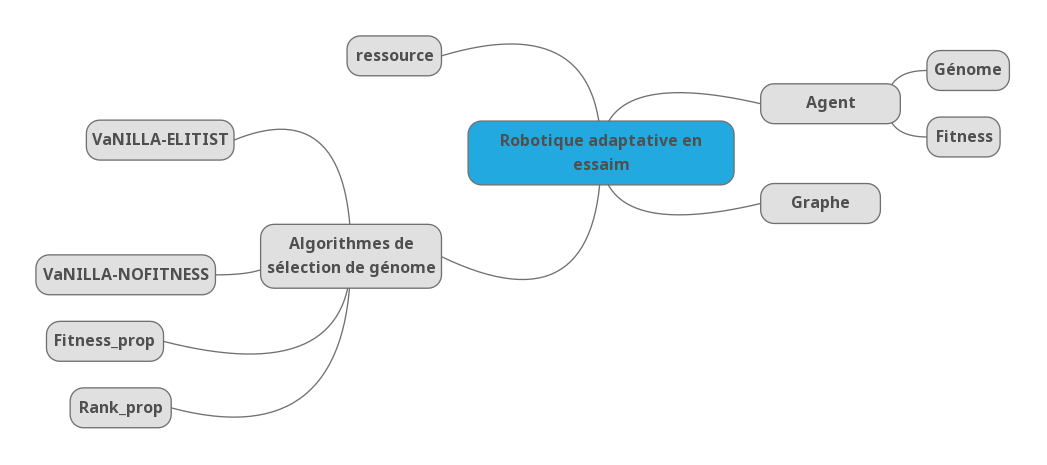
\includegraphics[scale=0.4]{carte.png} 

\section{Descriptif de la recherche documentaire}
   On a commencé notre recherche  par regarder les vidéos et les TDS  qui nous ont  permis de trouver les différents outils de recherche .Puis on a  lu  les articles fournis par notre encadrant pour  comprendre le sujet , ce qui  nous a aidé à déterminer  les mots clés .Par la suite on a utilisé Wikipédia pour déchiffrer ces mots clés  en langue française et anglaise .On s’est basé aussi sur le moteur de recherche Google permettant d’accéder à des pages web  à partir des mots clés ,titres et des questions qu’on se posait lors de notre recherche.On a utilisé aussi des outils académiques dans le domaine de la science et technologie tel que <web of science> ou on s’est inspiré des articles scientifiques,des livres et des synthèses  bibliographiques écrites par des chercheurs ou on peut sélectionner par date,auteur et type...
   
     Nous avons déduit que les articles scientifiques et académiques ont un niveau de spécialisation trop élevé ,se sont écrit par de chercheurs qui maîtrisent leurs domaines contrairement  aux outils de vulgarisation ou  se sont rédigés par des journalistes,vulgarisateurs .. qui ont un niveau de spécialisation pas élevé .


\section{Bibliographie produite dans le cadre du projet}
\end{flushleft}
\end{document}
